\newpage
\section{Auswertung}
\label{sec:Auswertung}
\subsection{Statische Methode}
\label{sec:Statische}
Aus den gemessenen Werten der statischen Methode bestimmt sich die Winkelrichtgröße nach Formel \eqref{eqn:D}, zu finden in Tabelle \ref{tab:D}.
\begin{align}
\intertext{Der Abstand von der Drehachse beträgt:}
 r=0,1375\,\si{\meter}.
\end{align}
Desweiteren wurden ein Fehler von $5°$für die Winkelmessung angenommen, da der Winkel nur durch fehlerbehaftetes Ablesen gemessen wurde.
Der in rad ungefähr $0,09$ rad beträgt.
Die errchneten Werte werden gemittelt und es ergibt sich eine Winkelrichtgröße von:
\begin{align}
  D=(0,044\pm0,010)\,\si{\newton\meter}
\end{align}
\begin{table}
 \centering
 \caption{Messwerte für die Federkonstante $D$ }
 \label{tab:D}
 \begin{tabular}{c c c}
\toprule
Auslenkwinkel $ \varphi\:/\:\text{rad} $      & $F\:/\:\si{\kilo\gram\meter\per\second\squared}$
& $D\:/\:\si{\kilo\gram\meter\squared\per\second\squared}$\\
\midrule
0,52\pm 0,09  &   0,09\pm 0,03   &   0,024\pm 0,008\\
0,87\pm 0,09  &   0,37\pm 0,03   &   0,058\pm 0,005\\
1,05\pm 0,09  &   0,38\pm 0,03   &   0,050\pm 0,004\\
1,22\pm 0,09  &   0,50\pm 0,03   &   0,056\pm 0,003\\
1,57\pm 0,09  &   0,52\pm 0,03   &   0,046\pm 0,003\\
2,09\pm 0,09  &   0,70\pm 0,03   &   0,046\pm 0,002\\
2,62\pm 0,09  &   0,75\pm 0,03   &   0,039\pm 0,002\\
3,14\pm 0,09  &   0,85\pm 0,03   &   0,037\pm 0,001\\
3,67\pm 0,09  &   0,95\pm 0,03   &   0,036\pm 0,001\\
4,19\pm 0,09  &   1,45\pm 0,03   &   0,048\pm 0,001\\
\bottomrule
\end{tabular}
\end{table}


\subsection{Dynamische Methode}
\label{sec:Dynamische}
Die Messwerte für die Dynamische Methode sind in dem Abb.\ref{abb:b} in der Form $T^2$ gegen $a^2$ aufgetragen.
Es besteht ein linearer Zusammenhang zwischen $T^2$ und $a^2$
wie in der Formel \eqref{eqn:cool}.
\begin{align}
I  &= 2(I_{\mathrm{z}}+m\cdot a^2) \\
D\cdot \frac{T^2}{4\pi^2}-I_{\mathrm{D}} &= 2(I_{\mathrm{z}}+m\cdot a^2)
\intertext{durch einstetzen der Formel \eqref{eqn:I} und umformen nach $a^2$ ergibt sich} %
a^2 &= D_{\mathrm{dyn}}\cdot \frac{T^2}{8\pi^2m}-\frac{I_{\mathrm{D}}}{2m}-\frac{I_{\mathrm{z}}}{m}\label{eqn:cool}
\intertext{Durch die Lineareregression lässt sich mit dem  Y-Achsenabschnitt  $a$ berechnen und somit durch Umformen  $I_{\mathrm{D}}$ bestimmen:}
a&=-\frac{I_{\mathrm{z}}}{m}-\frac{I_{\mathrm{D}}}{2m}\\
I_D&=-2ma-2I_z
\intertext{Durch einsetzten des Trägheitsmoments des Zylinders \eqref{eqn:zl} ergibt sich}
I_{\mathrm{D}}&=-2ma-2m\left(\frac{\left(\frac{d_{\mathrm{{z}}}}{2}\right)^2}{4}+\frac{h_{\mathrm{z}}^2}{12}\right)
\intertext{Durch Einsetzen der gemittelten gemessenen Größen}
 m&=(0,2225\pm0,000005)\, \si{\kilo\gram}\\
 d_{z1}&=(0,03494\pm0,00003)\,\si{meter}\\
H_z&=0,0300\pm0,00006\,\si{meter}
\intertext{ergibt sich für das Trägheitsmoment der Drillachse}
I_D&=(0,0027454\pm0,0000002)\,\si{\kilo\gram\meter\tothe{2}}
\intertext{Ebenfalls lässt sich mit Hilfe der aus der Linearenregression berechneten Steigung $b$ die dynamische Winkelrichtgröße $ D_\mathrm{dyn}$ bestimmen:  }
b=\frac{D_\mathrm{dyn}}{8\pi^2m}.\\
D_\mathrm{dyn}=8a\pi^2m.\\
\intertext{Durch einsetzen der Werte ergibt sich}
D_\mathrm{dyn}=(0,0295\pm0,0004)\, \si{\kilo\gram}.\\
\end{align}
Da sich die dynamische Winkelrichtgröße von der statisch gemessenen Winkelrichtgröße unterscheidet, wird die dynamische Winkelrichtgröße im
folgendem Teil als Winkelrichtgröße verwendet, da die folgenden Trägheitsmoment ebenfalls mit der Dynamischen Medthode bestimmt werden.
\begin{figure}
   \centering
   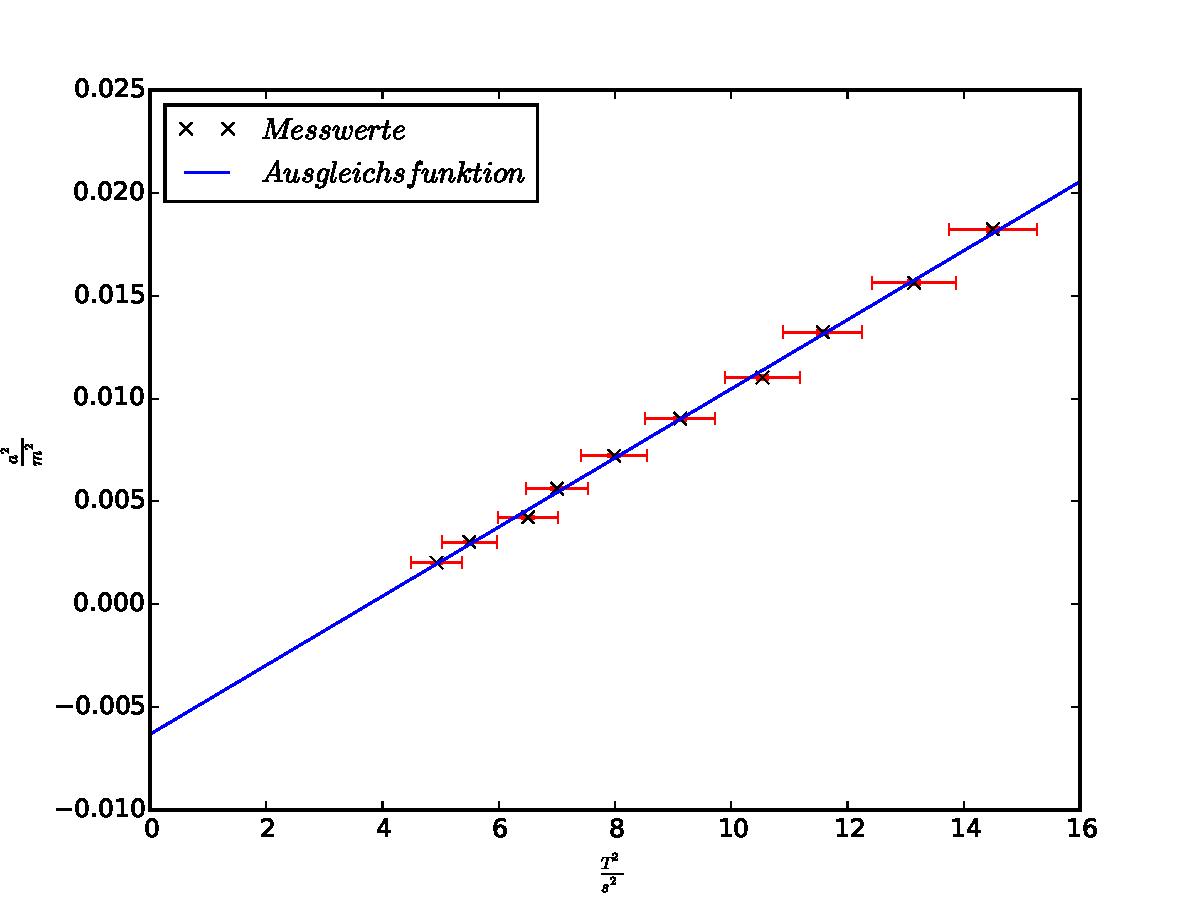
\includegraphics[width=0.7\textwidth]{b.pdf}
  \caption{Das Abstandsquadrat $a^2$ in Abhängigkeit von dem Periodendauerquadrat $T^2$ }
  \label{abb:b}
\end{figure}
\newpage
\subsection{Trägheitsmoment von geometrischen Figuren}
\subsubsection{Zylinder}
Nun werden die Werte für das Trägheitsmoment eines Zylinder,
mit der Masse
\begin{align*}
m=(1,9739\pm0,00005)\,\si{\meter}
\end{align*}
einmal mit der Formel  \eqref{eqn:I}
aus den Messwerten berechnet.
Dafür werden die gemessenen Zeiten gemittelt,
\begin{align*}
\overline{T}&= (1,455\pm0,016)\,\si{\second}\\
\intertext{und es ergibt sich ein}
I_{\mathrm{gemessen}}&=-(0,00116\pm0,00004)\,\si{\kilo\gram\meter\squared}.
\intertext{Das gemessene Trägheitsmoment ist laut
der Formel \eqref{eqn:I} negativ, da dies Physikalisch
nicht möglich ist, wird auf das Abziehen des Trägheitsmoment der Drillachse verzichtet.
Im Folgenden wird nun immer auf das Abziehen von $I_\mathrm{D}$ verzichtet,
da alle Trägheitsmomente sonst negativ werden.
Ohne Abziehen von $I_\mathrm{D}$ ergibt sich für das Trägheitsmoment der Zylinders:}
I_{\mathrm{gemessen}}&=(0,00158\pm0,00004)\,\si{\kilo\gram\meter\squared}.
\end{align*}
Aus der Theoretischenformel \eqref{eqn:zs} für
einen Zylinder der parallel zur Drehachse verläuft mit dem Durchmesser
\begin{align*}
  d_{z2}&=(0.08019\pm0.00011)\,\si{\meter},
\intertext{ergibt sich eine theoretisches Trägheitsmoment}
I_\mathrm{theorie}&= 0.0003011\pm0.0000006\,\si{\kilo\gram\meter\squared}.
\intertext{Somit beträgt die Abweichung von Theoriewerte die mit der Formel \eqref{eqn:abweich} berechnet wird}
a&=(425\pm13)\,\si{\percent}.
\end{align*}
\subsubsection{Kugel}
Dies mal wird das Trägheitsmoment eine Kugel,
die die Masse
\begin{align*}
m=(0,8125\pm0,00005)\si{\meter}
\end{align*}
besitzt, berechnet. Zuerst wird dieses wieder mit der Formel  \eqref{eqn:I}
aus den Messwerten bestimmt. Dafür werden
wieder die gemessenen Zeiten gemittelt,
\begin{align*}
  \overline{T}&=(1,486\pm0,007)\,\si{\second}
\intertext{und es ergibt sich ein}
I_\mathrm{gemessen}&=0,00165\pm0,00003)\,\si{\kilo\gram\meter\squared}.
\end{align*}
Aus der Theoretischenformel \eqref{eqn:Kugel} für eine
Kugel mit dem Durchmesser
\begin{align*}
  d_\mathrm{k}=(0,1365\pm0,0019)\,\si{\meter}
\end{align*}
ergibt sich ein theoretisches Trägheitsmoment von
\begin{align*}
I_{theorie}&=(0,00151\pm0,00004)\,\si{\kilo\gram\meter\squared}.
\intertext{Die relative Abweichung nach der Formel \eqref{eqn:abweich} beträgt somit:}
a&=(8,9\pm3,5)\,\si{\percent}.
\end{align*}
\newpage
\subsection{Trägheitsmoment einer Puppe}
Der Körper der Puppe wird mit verschiedenen
Zylindern genähert, wie in Abbildung \ref{fig:puppe}
 zu sehen ist.
\begin{figure}
 \centering
 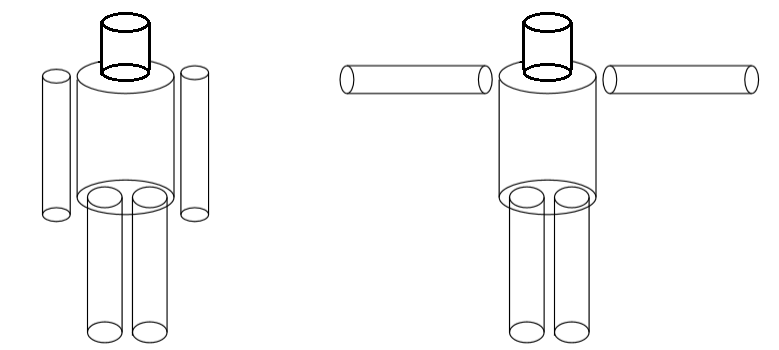
\includegraphics[width=0.3\textwidth]{puppe.PNG}
 \caption{Darstellung der Puppe mit Zylindern \cite{skript} }
 \label{fig:puppe}
 \end{figure}
Die gemessenen Werte werden gemittelt und es ergeben sich folgende Werte für die einzelnen Zylinder:
\begin{table}
  \centering
  \caption{Gemittelter Durchmesser und gemittelte Länge der einzelnen Zylinder}
  \label{tab:puppegemittelt}
  \begin{tabular}{c c c}
    \toprule
    $ $ & Höhe$/\si{\meter}$ & $Durchmesser / \si{\meter}$\\
    \midrule
    Beine & 0.2327\pm 0.0003 & 0.021\pm0.004 \\
    Arme  & 0.18
    1\pm 0.002 & 0.016\pm 0.003 \\
    Kopf  & 0.0772\pm 0.0.0005 & 0.03\pm 0.01 \\
    Torso & 0.122\pm 0.001 & 0.045\pm 0.008 \\
    \bottomrule
   \end{tabular}
\end{table}
\FloatBarrier
Mit der Masse der Puppe
\begin{align*}
  m_{\mathrm{ges}}= (0,3407\pm0,0005)\,\si{\kilo\gram}
\intertext{und dem gesamt Volumen }
V_{\mathrm{ges}}=(0,0005\pm0,0001)\,\si{\meter\tothe{3}}\\
\end{align*}
ergibt sich mit
\begin{align}
  \rho=\frac{m}{V}
\end{align}
\begin{align*}
\intertext{eine Dichte von}
\rho=(7,4\pm1,6)\,\si{\kilo\gram\meter\tothe{-3}}
\end{align*}
Mit diesen Ergebnissen lässt sich das theoretische Gesamtträgheitsmoment $I_\mathrm{gesTheo}$ bestimmen.
Dies ergibt sich aus den einzelnen Trägheitsmomenten der Zylinder, diese lassen sich mit Hilfe der Formel \eqref{eqn:zs}
und des Steinerschen Satzes bestimmen. Das Gesamtträgheitsmoment ergibt sich aus:
\begin{align}
  I_\mathrm{GesTheo}=I_\mathrm{Kopf}+I_\mathrm{Torso}+2\cdot I_\mathrm{Arm}+2\cdot I_\mathrm{Bein}
\end{align}
Die einzelnen Trägheitsmomente der Zylinder werden
mit Hilfe der Formel \eqref{eqn:zs} berechent.
Nur für die ausgestreckten Arme wird
die Formel \eqref{eqn:zl} benötigt.
Somit folgt für die einzelnen Trägheitsmomente mit angelegten Armen
\begin{align*}
I_\mathrm{Kopf} &=(0,0000022\pm0,0000041)\,\si{\kilo\gram\meter\squared},\\
I_\mathrm{Torso}&=(0,000037\pm0,000022)\,\si{\kilo\gram\meter\squared},\\
I_\mathrm{Arm}  &=(0,000026\pm0,000012)\,\si{\kilo\gram\meter\squared},\\
I_\mathrm{Bein} &=(0,0000093\pm0,0000057)\,\si{\kilo\gram\meter\squared}\\
\intertext{und somit ein Gesamtträgheitsmoment bei angelegten Armen von}
I_\mathrm{GesTheoAn}&=(0,000109\pm0,000030)\,\si{\kilo\gram\meter\squared}.\\
\intertext{Bei ausgestreckten Armen unterscheidet sich nur das Trägheitsmoment der Arme}
I_\mathrm{Arm}&=(0,00010\pm0,00004)\,\si{\kilo\gram\meter\squared}\\
\intertext{und als Gesamttägheitsmoment mit ausgestreckten Armen egibt sich}
I_\mathrm{GesTheoAus}&=(0,00089\pm0,00030)\,\si{\kilo\gram\meter\squared}\\
\end{align*}
Für das gemessene Gesamtträgheitmoment
müssen für beide Fälle
die gemessenen Zeiten gemittelt werden.
\begin{align*}
\overline{T}_\mathrm{an} &=(0,65\pm0,04)\,\si{\second}\\
\overline{T}_\mathrm{aus}&=(1.099\pm0.014)\,\si{\second}
\end{align*}
Diese Zeiten werden wieder in die Formel \eqref{eqn:I}
eingesetzt und es ergibt sich für den Fall das
die Arme angelegt sind eine Trägheitsmoment von:
\begin{align*}
I_\mathrm{GesMessAn}&=(0,00032\pm0,00004)\,\si{\kilo\gram\meter\squared}\\
\intertext{Für den Fall das die Puppe die Arme aussteckt:}
I_\mathrm{GesMessAus}&= (0,000903\pm0,000026)\,\si{\kilo\gram\meter\squared}.\\
\end{align*}
Der gemessenen Werte für den Fall, dass die Puppe die Arme angelegt hat,
weicht um
\begin{align*}
  a_\mathrm{An}=190\,\si{\percent}
\end{align*}
ab. Im Fall, dass die Puppe die Arme ausstreckt, ergibt sich
eine Abweichung von dem Theoriewerten von:
\begin{align*}
  a_\mathrm{Aus}=2\,\si{\percent}
\end{align*}
